%%=============================================================================
%% Methodologie
%%=============================================================================

\chapter{\IfLanguageName{dutch}{Methodologie}{Methodology}}%
\label{ch:methodologie}

%% TODO: In dit hoofstuk geef je een korte toelichting over hoe je te werk bent
%% gegaan. Verdeel je onderzoek in grote fasen, en licht in elke fase toe wat
%% de doelstelling was, welke deliverables daar uit gekomen zijn, en welke
%% onderzoeksmethoden je daarbij toegepast hebt. Verantwoord waarom je
%% op deze manier te werk gegaan bent.
%% 
%% Voorbeelden van zulke fasen zijn: literatuurstudie, opstellen van een
%% requirements-analyse, opstellen long-list (bij vergelijkende studie),
%% selectie van geschikte tools (bij vergelijkende studie, "short-list"),
%% opzetten testopstelling/PoC, uitvoeren testen en verzamelen
%% van resultaten, analyse van resultaten, ...
%%
%% !!!!! LET OP !!!!!
%%
%% Het is uitdrukkelijk NIET de bedoeling dat je het grootste deel van de corpus
%% van je bachelorproef in dit hoofstuk verwerkt! Dit hoofdstuk is eerder een
%% kort overzicht van je plan van aanpak.
%%
%% Maak voor elke fase (behalve het literatuuronderzoek) een NIEUW HOOFDSTUK aan
%% en geef het een gepaste titel.

Dit hoofdstuk bespreekt kort de fasen van het onderzoek. Per fase word kort besproken wat de doelstelling is en welke keuzes gemaakt werden. In Figuur 3.1 wordt een overzicht getoond van de verschillende fasen en hoe deze elkaar opvolgen.
\begin{figure}
	\centering
	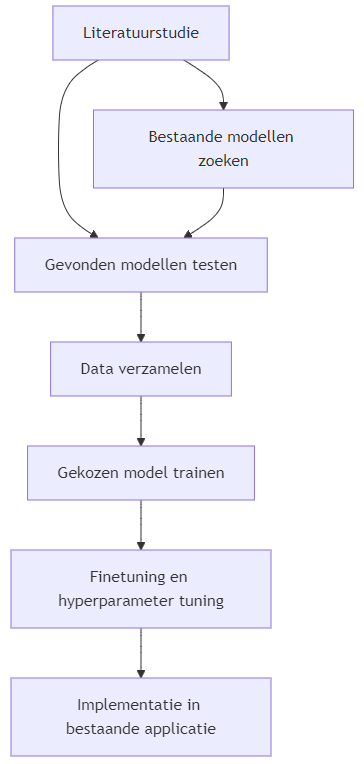
\includegraphics[width=\columnwidth]{./img/verloop.png}
	\caption{Voorstelling van de fasen van de bachelorproef en hun onderlinge volgorde}
\end{figure}


\paragraph{Literatuurstudie en modellen kiezen}
Deze fase bestaat uit het opzoeken van info omtrent diarization en welke bestaande modellen hier al voor zijn. Hieruit worden de modellen gekozen die het meeste potentieel lijken te hebben om tot een goed eindresultaat te komen en wordt gekeken wat de beste manier van aanpakken is.\\
Naast het zoeken naar modellen, wordt ook gezocht naar methoden om deze modellen te evalueren. Dit zorgt ervoor dat er een gegronde keuze kan gemaakt worden om verder te gaan met een specifiek model. Dit zorgt er in een latere fase ook voor dat er gekozen kan worden voor de beste parameters voor het model.

\paragraph{Modellen trainen}
In deze fase worden de modellen die in de eerste fase gekozen werden getraind met Vlaamse audiofragmenten. 
%TODO 

\paragraph{Finetunen en evalueren}
In deze fase worden de getrainde modellen uit voorgaande fase geëvalueerd aan de hand van evaluatiemethoden die gevonden werden in de eerste fase. Op basis hiervan wordt het model gekozen dat de beste resultaten oplevert.\\
Na het maken van de keuze worden de parameters van het gekozen model gefinetuned om zo het best mogelijke resultaat te kunnen bekomen. Voor dit finetunen zal ook gebruikt gemaakt worden van de evaluatiemethoden die eerder vermeld werden.

\paragraph{Implementatie in de applicatie}
In deze fase zal het model opgeslagen worden en geïmplementeerd worden in de broncode van de reeds bestaande applicatie. Er zal ook grondig getest worden of het model hierin het beoogde resultaat heeft.